%===============================================================================
% LaTeX sjabloon voor de bachelorproef toegepaste informatica aan HOGENT
% Meer info op https://github.com/HoGentTIN/latex-hogent-report
%===============================================================================

\documentclass[dutch,dit,thesis]{hogentreport}

% TODO:
% - If necessary, replace the option `dit`' with your own department!
%   Valid entries are dbo, dbt, dgz, dit, dlo, dog, dsa, soa
% - If you write your thesis in English (remark: only possible after getting
%   explicit approval!), remove the option "dutch," or replace with "english".

\usepackage{lipsum} % For blind text, can be removed after adding actual content

%% Pictures to include in the text can be put in the graphics/ folder
\graphicspath{{../graphics/}}

%% For source code highlighting, requires pygments to be installed
%% Compile with the -shell-escape flag!
%% \usepackage[chapter]{minted}
%% If you compile with the make_thesis.{bat,sh} script, use the following
%% import instead:
\usepackage[chapter,outputdir=../output]{minted}
\usemintedstyle{solarized-light}

%% Formatting for minted environments.
\setminted{%
    autogobble,
    frame=lines,
    breaklines,
    linenos,
    tabsize=4
}

%% Ensure the list of listings is in the table of contents
\renewcommand\listoflistingscaption{%
    \IfLanguageName{dutch}{Lijst van codefragmenten}{List of listings}
}
\renewcommand\listingscaption{%
    \IfLanguageName{dutch}{Codefragment}{Listing}
}
\renewcommand*\listoflistings{%
    \cleardoublepage\phantomsection\addcontentsline{toc}{chapter}{\listoflistingscaption}%
    \listof{listing}{\listoflistingscaption}%
}

% Other packages not already included can be imported here

%%---------- Document metadata -------------------------------------------------
% TODO: Replace this with your own information
\author{Ernst Aarden}
\supervisor{Dhr. F. Van Houte}
\cosupervisor{Mevr. S. Beeckman}
\title[Optionele ondertitel]%
    {Titel van de bachelorproef}
\academicyear{\advance\year by -1 \the\year--\advance\year by 1 \the\year}
\examperiod{1}
\degreesought{\IfLanguageName{dutch}{Professionele bachelor in de toegepaste informatica}{Bachelor of applied computer science}}
\partialthesis{false} %% To display 'in partial fulfilment'
%\institution{Internshipcompany BVBA.}

%% Add global exceptions to the hyphenation here
\hyphenation{back-slash}

%% The bibliography (style and settings are  found in hogentthesis.cls)
\addbibresource{bachproef.bib}            %% Bibliography file
\addbibresource{../voorstel/voorstel.bib} %% Bibliography research proposal
\defbibheading{bibempty}{}

%% Prevent empty pages for right-handed chapter starts in twoside mode
\renewcommand{\cleardoublepage}{\clearpage}

\renewcommand{\arraystretch}{1.2}

%% Content starts here.
\begin{document}

%---------- Front matter -------------------------------------------------------

\frontmatter

\hypersetup{pageanchor=false} %% Disable page numbering references
%% Render a Dutch outer title page if the main language is English
\IfLanguageName{english}{%
    %% If necessary, information can be changed here
    \degreesought{Professionele Bachelor toegepaste informatica}%
    \begin{otherlanguage}{dutch}%
       \maketitle%
    \end{otherlanguage}%
}{}

%% Generates title page content
\maketitle
\hypersetup{pageanchor=true}

%%=============================================================================
%% Voorwoord
%%=============================================================================

\chapter*{\IfLanguageName{dutch}{Woord vooraf}{Preface}}%
\label{ch:voorwoord}

Toen ik op het forum voor potentiële bachelorproefonderwerpen dit project rond computer visie in het Zorglab zag, was mijn interesse onmiddellijk gewekt. 
Na enkele jaren professioneel actief te zijn in de wereld van computer vision, zag ik hierin een unieke kans om 
mijn technische vaardigheden in te zetten voor een maatschappelijk relevant doel.
Bovendien bood het een gelegenheid om meer te leren over de nuances en valkuilen binnen de zorgverlening – een wereld die tot dan toe relatief onbekend voor me was.

Het zaadje waaruit dit project is gegroeid, werd geplant door dhr. Jorrit Campens, lector en onderzoeker aan HOGENT en een drijvende kracht achter het Zorglab.
Zijn domeinexpertise in de zorg vormde een perfecte aanvulling op mijn technische achtergrond. 
Onze samenwerking voelde als een natuurlijke synergie, waarbij hij me doorheen het hele traject, van gerichte feedback voorzag.
Ik herinner me nog goed ons eerste gesprek in het Zorglab, waarbij dhr. Campens zijn droom schetste van een geautomatiseerde analysemethode voor observaties in zorgsimulaties.
Hij omschreef het toen als `naar de maan gaan', een uitdaging die me meteen aansprak. Voor zijn enthousiasme en stimulans, ben ik hem dan ook bijzonder dankbaar.

Toegegeven, het project was ambitieus en uitdagend, zeker in combinatie met mijn deeltijdse werk als softwareontwikkelaar gedurende het semester.
Desondanks zag ik het als een perfecte kans om de diverse vaardigheden die ik doorheen de jaren heb opgebouwd, samen te brengen.
Mijn IT-reis begon met het ontwikkelen van games in het middelbaar en evolueerde naar het bouwen van webapplicaties en het verkennen van frontend-tecnologieën.
Binnen mijn opleiding aan HOGENT koos ik bewust voor de minor Data \& AI, een domein waarin ik mijn kennis nog verder in wilde verdiepen.
Deze bachelorproef voelde dan ook als een culminatiepunt, waar ik mijn passie voor frontend, backend en data science kon verenigen.

Mijn dank gaat ook uit naar mijn promotor, dhr. Bert Van Vreckem, voor zijn waardevolle inhoudelijke feedback en zijn beschikbaarheid voor overlegmomenten gedurende het traject.
Een speciaal woord van dank wil ik richten aan mijn bonusvader, Dirk Coussement.
Als auteur voor een lokaal blad heeft hij een scherp oog voor taal en heeft hij mij enorm geholpen bij het nalezen van deze bachelorproef.

Tenslotte wil ik ook de studenten bedanken die de tijd namen om deel te nemen aan het experiment in het Zorglab. 
Zonder hun medewerking was het verzamelen van de nodige data niet mogelijk geweest.

Ik hoop dat deze bachelorproef een bruikbare eerste stap vormt naar een meer objectieve en efficiënte manier om observatievaardigheden in zorgopleidingen te evalueren.
%%=============================================================================
%% Samenvatting
%%=============================================================================

\IfLanguageName{english}{%
\selectlanguage{dutch}
\chapter*{Samenvatting}


\selectlanguage{english}
}{}

%%---------- Samenvatting -----------------------------------------------------
% De samenvatting in de hoofdtaal van het document

\chapter*{\IfLanguageName{dutch}{Samenvatting}{Abstract}}

Observatievaardigheden zijn van belang voor zorgverleners, zowel voor accurate diagnoses als voor empathische patiëntondersteuning. 
De huidige evaluatie van deze vaardigheden in gesimuleerde omgevingen steunt vaak op subjectieve 
methoden zoals zelfrapportage en directe observatie door docenten. 
Hoewel de Tobii eyetracking-brillen in het Zorglab van HOGENT objectieve blikdata leveren, 
ontbreekt er tot op heden geschikte software om automatisch te analyseren welke objecten studenten waarnemen en voor hoe lang. 
Deze bachelorproef beantwoordt hoe computervisiemodellen geïntegreerd kunnen worden met 
eyetrackingdata van Tobii Glasses om de observatieprestaties van studenten automatisch te analyseren.
De analyses dienen de feedback door docenten in het Zorglab te versterken.

Deze doelstelling werd uitgewerkt door middel van van een proof-of-concept (PoC) softwareapplicatie. 
Dit proces startte met een literatuurstudie naar eyetracking-analyse en relevante computervisiemodellen (o.a. YOLO, SAM, DINOv2). 
Vervolgens werd een prototype applicatie ontworpen en geïmplementeerd (Python, FastAPI, HTMX), 
inclusief een semi-automatische labeling-tool die gebruik maakt van SAM2 voor objectsegmentatie en -tracking. 
Om de PoC te valideren, werd een gecontroleerd experiment uitgevoerd in het Zorglab. 
Hier genereerden studenten aan de hand van Tobii Pro Glasses 3, eyetrackingopnames tijdens gesimuleerde observatietaken. 
Deze opnames, samen met twee specifieke kalibratieopnames, werden gelabeld met de ontwikkelde tool om een grondwaarheidsdataset te creëren. 
Een analysepijplijn werd ontworpen en geëvalueerd. In deze analyse werd de trackingfunctionaliteit van FastSAM gecombineerd met 
blikgestuurde filtering en classificatie van objectsegmenten, middels een getraind YOLOv11-objectdetectiemodel. 
De prestaties werden geëvalueerd aan de hand van precisie, recall en F1-score, na optimalisatie via een grid search van hyperparameters.

Uit de resultaten bleek dat de combinatie van FastSAM-tracking met een YOLOv11-objectdetector (getraind op 1000 samples per klasse) 
de beste prestaties opleverde, met een F1-score van 0.80, een precisie van 0.94 en een recall van 0.70. 
De hoge precisie toont aan dat het systeem met grote zekerheid de correcte objecten identificeert, 
hoewel een significant deel van de fout-positieven in de werkelijkheid correct gedetecteerde objecten bleken te zijn, die niet in de grondwaarheid waren opgenomen. 
De lagere recall wijst erop dat niet alle bekeken objecten consistent werden gedetecteerd, voornamelijk door problemen met kleine, 
transparante objecten en door inconsistenties tussen de FastSAM-segmentaties en de grondwaarheid. 
De FastSAM-tracking bleek de meest beperkende factor in de pijplijn.

Deze bachelorproef levert een werkend PoC en een methodologie op die de haalbaarheid van geautomatiseerde 
analyse van observatievaardigheden aantoont.\\
Het biedt een objectieve, datagestuurde basis om de feedback aan studenten te verbeteren en de effectiviteit van simulatietraining in de zorg te verhogen.
Op deze manier legt het een fundament voor verder onderzoek naar robuustere analysemethoden.

%---------- Inhoud, lijst figuren, ... -----------------------------------------

\tableofcontents

% In a list of figures, the complete caption will be included. To prevent this,
% ALWAYS add a short description in the caption!
%
%  \caption[short description]{elaborate description}
%
% If you do, only the short description will be used in the list of figures

\listoffigures

% If you included tables and/or source code listings, uncomment the appropriate
% lines.
\listoftables

\listoflistings

% Als je een lijst van afkortingen of termen wil toevoegen, dan hoort die
% hier thuis. Gebruik bijvoorbeeld de ``glossaries'' package.
% https://www.overleaf.com/learn/latex/Glossaries

%---------- Kern ---------------------------------------------------------------

\mainmatter{}

% De eerste hoofdstukken van een bachelorproef zijn meestal een inleiding op
% het onderwerp, literatuurstudie en verantwoording methodologie.
% Aarzel niet om een meer beschrijvende titel aan deze hoofdstukken te geven of
% om bijvoorbeeld de inleiding en/of stand van zaken over meerdere hoofdstukken
% te verspreiden!

%%=============================================================================
%% Inleiding
%%=============================================================================

\chapter{\IfLanguageName{dutch}{Inleiding}{Introduction}}%
\label{ch:inleiding}

Observatievaardigheden van zorgverleners zijn niet enkel belangrijk om nauwkeurige diagnoses te stellen, maar ook om de patiënt te ondersteunen en te begeleiden. 
Zo zien we dat studenten in de ouderenzorg vaak moeite hebben met sociale omgang en communicatie met ouderen. 
In het 360° Zorglab aan HOGENT worden studenten getraind via simulaties waarbij ze in een omgeving zoals een ziekenhuis kamer of woonkamer geplaatst worden.
Zo leren ze de nuances van zorgverlening kennen en worden ze geconfonteerd met concrete situaties. 
Een belangrijk aspect van deze training is dat studenten leren om kritische objecten, zoals een colafles op het nachtkastje van een diabetespatiënt, op te merken.
Tot op heden wordt er gesteund op zelfrapportage en observatie door docenten om de vaardigheden van de sudenten te evalueren.
Echter is dit een subjectieve methode die niet altijd even betrouwbaar is, waardoor er nood is aan een objectievere methode om observatievaardigheden te evalueren.
Het Zorglab beschikt over een Tobii eyetracking-bril die de oogbewegingen van de studenten kunnen registreren, en een camera bezit die het gezichtsveld van de studenten kan opnemen.
Eerder werk richtte zich op het visualiseren van het pad waarlangs de blik van de studenten beweegt, maar zo steunt de analyse op het herbekijken van elke opname.
Bovendien produceert deze methode geen bruikbare metrieken die de prestaties van de studenten objectief kunnen becijferen.
Hierdoor is er een nood aan een geautomatiseerde methode om de eyetrackingdata te analyseren en te visualiseren, zodat trainers snel inzicht krijgen in de observatieprestaties van studenten.

\section{\IfLanguageName{dutch}{Probleemstelling}{Problem Statement}}%
\label{sec:probleemstelling}

Hoewel de Tobii Glasses bruikbare data opleveren, ontbreekt er momenteel geschikte software om te analyseren of studenten daadwerkelijk naar deze objecten hebben gekeken.
Dit gebrek aan dataverwerking en visualisatie maakt het voor trainers lastig om de observatieprestaties van studenten efficiënt te beeordelen en te verbeteren.
Zonder een geautomatiseerde manier om te detecteren welke specifieke objecten studenten wel of niet hebben waargenomen, wordt het geven van directe feedback een tijdrovend proces. 

\section{\IfLanguageName{dutch}{Onderzoeksvraag}{Research question}}%
\label{sec:onderzoeksvraag}

Hoe kunnen computervisie-modellen geïntegreerd worden met eyetrackingdata van Tobii Glasses om observatieprestaties van studenten in het 360° Zorglab automatisch te analyseren en te visualiseren?
Deze onderzoeksvraag wordt uitgewerkt aan de hand van de volgende deelvragen:
\begin{itemize}
    \item Welke barrières (cognitief, technisch of didactisch) ervaren trainers en studenten bij de huidige, handmatige observatiemethode?
    \item Welke bestaande objectdetectie en segmentatie modellen zijn hiervoor geschikt?
    \item Hoe kan een softwareoplossing ontwikkeld worden voor een gebruiksvriendelijke analyse en visualisatie van de eyetrackingdata?
    \item In welke mate kunnen de modellen en de ontwikkelde software:
        \begin{enumerate}
            \item correct bepalen welke kritische objecten studenten hebben waargenomen?
            \item nauwkeurig meten hoe lang studenten naar deze objecten kijken?
        \end{enumerate}
\end{itemize}

\section{\IfLanguageName{dutch}{Onderzoeksdoelstelling}{Research objective}}%
\label{sec:onderzoeksdoelstelling}

Het doel is om trainers in het Zorglab te ondersteunen bij het analyseren en visualiseren van eyetrackingdata, zodat ze snel inzicht krijgen in de observatieprestaties van studenten en kunnen 
vaststellen of belangrijke objecten tijdens zorgsimulaties zijn waargenomen. Er zullen hiervoor twee metrieken worden berekend: naar welke objecten de studenten kijken en hoe lang ze naar deze objecten kijken.
Hiervoor wordt een proof-of-concept softwareoplossing ontwikkeld die de eyetrackingdata van Tobii Glasses combineert met objectdetectie- en segmentatiemodellen op een gebruiksvriendelijke manier.
Ook wordt er onderzocht hoe accuraat het uiteindelijke systeem is in het berekenen van de metrieken.

\section{\IfLanguageName{dutch}{Opzet van deze bachelorproef}{Structure of this bachelor thesis}}%
\label{sec:opzet-bachelorproef}

% Het is gebruikelijk aan het einde van de inleiding een overzicht te
% geven van de opbouw van de rest van de tekst. Deze sectie bevat al een aanzet
% die je kan aanvullen/aanpassen in functie van je eigen tekst.

De rest van deze bachelorproef is als volgt opgebouwd:

In Hoofdstuk~\ref{ch:stand-van-zaken} wordt een overzicht gegeven van de stand van zaken binnen het onderzoeksdomein, op basis van een literatuurstudie.

In Hoofdstuk~\ref{ch:methodologie} wordt de methodologie toegelicht en worden de gebruikte onderzoekstechnieken besproken om een antwoord te kunnen formuleren op de onderzoeksvragen.

In Hoofdstuk~\ref{ch:ontwikkeling} wordt de ontwikkeling van de proof-of-concept applicatie toegelicht.

In Hoofdstuk~\ref{ch:experiment} wordt het experimenteel onderzoek besproken dat werd uitgevoerd om de proof-of-concept applicatie te evalueren.

In Hoofdstuk~\ref{ch:analyse-en-resultaten} worden de experimentele opnames geanalyseerd en de resultaten besproken.

In Hoofdstuk~\ref{ch:conclusie}, tenslotte, wordt de conclusie gegeven en een antwoord geformuleerd op de onderzoeksvragen. Daarbij wordt ook een aanzet gegeven voor toekomstig onderzoek binnen dit domein.
\chapter{\IfLanguageName{dutch}{Stand van zaken}{State of the art}}%
\label{ch:stand-van-zaken}

% Tip: Begin elk hoofdstuk met een paragraaf inleiding die beschrijft hoe
% dit hoofdstuk past binnen het geheel van de bachelorproef. Geef in het
% bijzonder aan wat de link is met het vorige en volgende hoofdstuk.

% Pas na deze inleidende paragraaf komt de eerste sectiehoofding.

Dit hoofdstuk bevat je literatuurstudie. De inhoud gaat verder op de inleiding, maar zal het onderwerp van de bachelorproef *diepgaand* uitspitten. De bedoeling is dat de lezer na lezing van dit hoofdstuk helemaal op de hoogte is van de huidige stand van zaken (state-of-the-art) in het onderzoeksdomein. Iemand die niet vertrouwd is met het onderwerp, weet nu voldoende om de rest van het verhaal te kunnen volgen, zonder dat die er nog andere informatie moet over opzoeken \autocite{Pollefliet2011}.

Je verwijst bij elke bewering die je doet, vakterm die je introduceert, enz.\ naar je bronnen. In \LaTeX{} kan dat met het commando \texttt{$\backslash${textcite\{\}}} of \texttt{$\backslash${autocite\{\}}}. Als argument van het commando geef je de ``sleutel'' van een ``record'' in een bibliografische databank in het Bib\LaTeX{}-formaat (een tekstbestand). Als je expliciet naar de auteur verwijst in de zin (narratieve referentie), gebruik je \texttt{$\backslash${}textcite\{\}}. Soms is de auteursnaam niet expliciet een onderdeel van de zin, dan gebruik je \texttt{$\backslash${}autocite\{\}} (referentie tussen haakjes). Dit gebruik je bv.~bij een citaat, of om in het bijschrift van een overgenomen afbeelding, broncode, tabel, enz. te verwijzen naar de bron. In de volgende paragraaf een voorbeeld van elk.

\textcite{Knuth1998} schreef een van de standaardwerken over sorteer- en zoekalgoritmen. Experten zijn het erover eens dat cloud computing een interessante opportuniteit vormen, zowel voor gebruikers als voor dienstverleners op vlak van informatietechnologie~\autocite{Creeger2009}.

Let er ook op: het \texttt{cite}-commando voor de punt, dus binnen de zin. Je verwijst meteen naar een bron in de eerste zin die erop gebaseerd is, dus niet pas op het einde van een paragraaf.

\begin{figure}
  \centering
  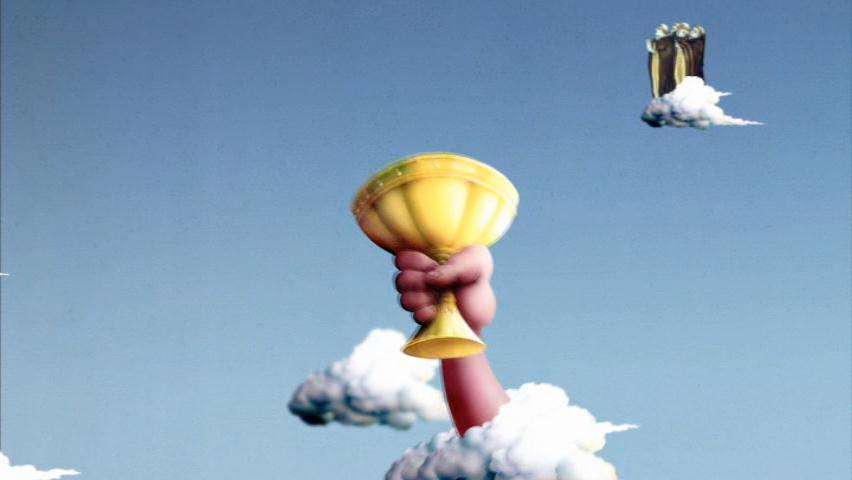
\includegraphics[width=0.8\textwidth]{grail.jpg}
  \caption[Voorbeeld figuur.]{\label{fig:grail}Voorbeeld van invoegen van een figuur. Zorg altijd voor een uitgebreid bijschrift dat de figuur volledig beschrijft zonder in de tekst te moeten gaan zoeken. Vergeet ook je bronvermelding niet!}
\end{figure}

\begin{listing}
  \begin{minted}{python}
    import pandas as pd
    import seaborn as sns

    penguins = sns.load_dataset('penguins')
    sns.relplot(data=penguins, x="flipper_length_mm", y="bill_length_mm", hue="species")
  \end{minted}
  \caption[Voorbeeld codefragment]{Voorbeeld van het invoegen van een codefragment.}
\end{listing}

\lipsum[7-20]

\begin{table}
  \centering
  \begin{tabular}{lcr}
    \toprule
    \textbf{Kolom 1} & \textbf{Kolom 2} & \textbf{Kolom 3} \\
    $\alpha$         & $\beta$          & $\gamma$         \\
    \midrule
    A                & 10.230           & a                \\
    B                & 45.678           & b                \\
    C                & 99.987           & c                \\
    \bottomrule
  \end{tabular}
  \caption[Voorbeeld tabel]{\label{tab:example}Voorbeeld van een tabel.}
\end{table}


%%=============================================================================
%% Methodologie
%%=============================================================================

\chapter{\IfLanguageName{dutch}{Methodologie}{Methodology}}%
\label{ch:methodologie}

Het onderzoek werd uitgevoerd in een iteratieve cyclus, waarbij de verschillende fasen van het project elkaar opvolgden en elkaar beïnvloedden.
Deze sectie beschrijft in grote lijnen de verschillende fasen van het onderzoek, de doelstellingen en de gebruikte methodologieën.
Figuur~\ref{fig:methodologie} toont een flowchart van de methodologie, waarin de verschillende fasen en hun onderlinge relaties worden weergegeven.
De labels op de pijlen geven de belangrijkste deliverables van elke fase aan, die als input dienen voor de volgende fase(s).
\begin{figure}[H]
  \centering
  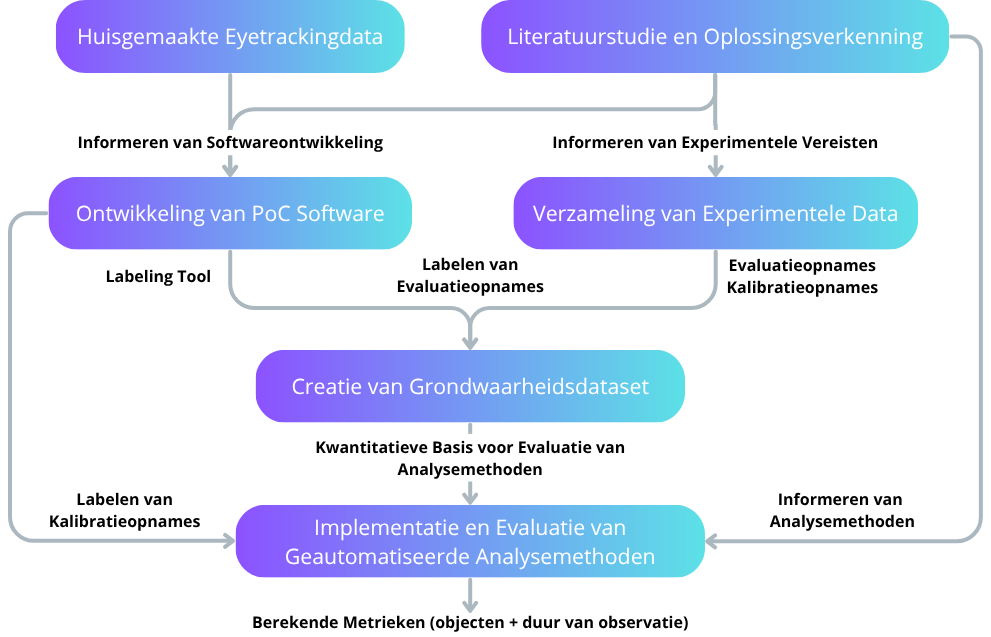
\includegraphics[width=0.9\textwidth]{methodologie.png}
  \caption{Flowchart van de methodologie van het onderzoek.}
  \label{fig:methodologie}
\end{figure}

\section{Literatuurstudie}

De literatuurstudie vormde een iteratief proces gedurende het gehele onderzoek, beginnend met een brede initiële verkenning en 
later verfijnd en aangevuld naarmate specifieke vragen tijdens het project opdoken. 
Het overkoepelende doel was een grondig en actueel inzicht te verwerven in de relevante domeinen. 
Hierbij lag de focus op de volgende gebieden: 
\begin{enumerate}
  \item Onderzoeken hoe de evaluatie van observatieprestaties momenteel wordt uitgevoerd, met bijzondere aandacht aan de nood aan een geautomatiseerde aanpak.
  \item De huidige stand van zaken in eyetracking-technologie, met aandacht voor hoofd-gemonteerde systemen zoals de Tobii Pro Glasses 3 en de analyse van de hieruit voortkomende data.
  \item State-of-the-art technieken binnen Computer Vision, waaronder objectdetectie (bv. YOLO, DETR, Grounding DINO), segmentatie (bv. Mask R-CNN, SAM, FastSAM) en image embedding (bv. CLIP, DINOv2).
  \item Bestaande integraties van eyetracking en Computer Vision.
\end{enumerate}
Wetenschappelijke publicaties, technische documentatie en relevante open-sour\-ce projecten werden hiervoor systematisch 
geraadpleegd en kritisch geanalyseerd.
Hoofdstuk~\ref{ch:stand-van-zaken} beschrijft uitvoerig de bevindingen van deze literatuurstudie.

\section{Oplossingsverkenning}

Voortbouwend op de inzichten uit de literatuurstudie, richtte de tweede fase zich op het verkennen en evalueren van verschillende 
conceptuele oplossingsstrategieën om de centrale onderzoeksvraag te beantwoorden. 
Het doel was om een reeks potentiële benaderingen te formuleren voor het automatisch analyseren 
van eyetrackingdata in combinatie met computervisiemodellen, en hieruit de meest veelbelovende te 
selecteren voor de ontwikkeling van de Proof-of-Concept (PoC). 
Dit proces omvatte het conceptueel ontwerpen van diverse pipelines, waarbij de inputs (eyetracking-opnames, objectdefinities) 
en de gewenste outputs (geobserveerde objecten, observatieduur) als leidraad dienden. 
De strategieën varieerden op vlak van algemene aanpak, de typen computervisiemodellen 
en de rol van de blikdata in het proces. 
Elke strategie werd kwalitatief beoordeeld op criteria zoals verwachte accuraatheid, complexiteit van implementatie, 
computationele vereisten en flexibiliteit. 
Deze analyse resulteerde in een beargumenteerde keuze voor de strategie die als basis diende voor het onderzoek, 
zoals gedetailleerd in Hoofdstuk~\ref{ch:oplossingsstrategieen}.

\section{Huisgemaakte Eyetrackingdata}

Voor het onderzoek en het uitwerken van de PoC software-applicatie, was het belangrijk om zicht te krijgen op de werking van de Eyetracker en de bijhorende software.
Daarom werd deze ontleend uit het Zorglab van HoGent voor een periode van 3 weken. 
Tijdens deze periode werden thuis verschillende opnames gemaakt in een woonkamer met diverse objecten, met de volgende specifieke doelstellingen:
\begin{itemize}
    \item Het leren werken met de Tobii Pro Glasses 3 en de bijhorende software.
    \item Nagaan hoe men de eyetrackingdata kan exporteren naar een bruikbaar formaat via de WiFi-verbinding van de eyetracker.
    \item Een dataset creëren die kan dienen als basis voor het uitwerken van de PoC.
\end{itemize}
Deze opnames werden niet gebruikt voor de uiteindelijke evaluatie van de PoC, aangezien de data afkomstig zijn van tests waarbij de onderzoeker zelf de eyetracker droeg.
Hierdoor is er sprake van mogelijke bias, wat de objectiviteit van de data in het gedrang brengt.

\section{Proof of Concept Software Applicatie}

Een kernonderdeel van deze bachelorproef was de ontwikkeling van een Proof-of-Concept (PoC) softwareapplicatie. 
Het hoofddoel van deze fase was het ontwerpen en implementeren van een werkend prototype dat de beoogde workflow ondersteunt: van het importeren van ruwe eyetracking-opnames tot het genereren van gelabelde data die als basis kan dienen voor analyse. 
De methodologie omvatte de selectie van een passende, moderne technologie-stack (o.a. Python, FastAPI, HTMX, SQLite) gericht op modulariteit en toekomstige uitbreidbaarheid. 
Een significant onderdeel was het ontwerp en de implementatie van een semi-automatische labeling-tool, bedoeld om de efficiëntie van het labelingsproces te verhogen. 
Er werd ingezet op duurzame software-ontwikkelpraktijken zoals type hinting en containerisatie (Docker) om de mogelijkheid tot onderhoud en reproduceerbaarheid te waarborgen. 
De resulterende applicatie, inclusief de architectuur, componenten en technische keuzes, wordt uitvoerig beschreven in Hoofdstuk~\ref{ch:ontwikkeling}.

\section{Experimenteel Onderzoek}

Zoals eerder vermeld, werd de thuisopgenomen dataset niet gebruikt voor de evaluatie van de PoC. 
Om een onbevooroordeelde dataset te verkrijgen en om de modaliteiten van de uitwerking te valideren (bijvoorbeeld: invloed van de afstand tussen de Eyetracker en het object, en de aard van de objecten), werd er een gecontroleerd experiment opgezet in het Zorglab van HoGent.
Het doel van dit experiment was om een dataset te creëren die als grond-waarheid diende voor de metrieken die de PoC berekent (bekeken objecten en tijdsduur).
Op de campus werden studenten van diverse opleidingen gevraagd om deel te nemen aan het experiment.
De 14 resulterende opnames werden daarna gelabeld via de labeling-tool van de PoC, met een manuele kwaliteitscontrole om de betrouwbaarheid van de data te waarborgen.
Voor een uitgebreide beschrijving van het opzet en de uitvoering van het experiment, inclusief de gebruikte methodologieën, wordt verwezen naar Hoofdstuk~\ref{ch:experiment}.

\section{Creatie van een Grondwaarheidsdataset}

Om de prestaties van de geautomatiseerde analysemethoden objectief te kunnen evalueren, was de creatie van een nauwkeurige 
grondwaarheidsdataset noodzakelijk. Het doel van deze fase was om, voor elke evaluatieopname uit het experiment, 
frame-per-frame vast te stellen welke van de 15 gedefinieerde objecten daadwerkelijk door de deelnemer werden bekeken. 
De methodologie startte met het voorbereiden van de ruwe opnamedata (video en blikdata). 
Vervolgens werden de evaluatieopnames gelabeld met behulp van de ontwikkelde labeling-tool (zie Hoofdstuk~\ref{ch:ontwikkeling}).
Hierbij segmenteerde de onderzoeker objecten waar de blik van de deelnemer op rustte, met behulp van het SAM2-model en de trackingfunctionaliteit van de labeling-tool.
Deze initiële segmentaties werden daarna gefilterd op basis van de geregistreerde blikpunten, waarbij een cirkelvormig kijkgebied moest overlappen met het segmentatiemasker. 
Dit resulteerde in een dataset die per frame de bekeken objecten, hun bounding boxes en maskeroppervlakte specificeert. 
De correctheid werd manueel gevalideerd. De gedetailleerde stappen van dit proces zijn beschreven in Hoofdstuk~\ref{ch:grondwaarheid}.

\section{Analyse van Observatieprestaties}

De laatste fase van het onderzoek focuste op het implementeren en evalueren van een geautomatiseerde analysepipeline om observatieprestaties te meten, 
conform de gekozen oplossingsstrategie (Strategie 4 uit Hoofdstuk~\ref{ch:oplossingsstrategieen}). 
Het doel was om automatisch te bepalen welke kritische objecten werden waargenomen en hoe lang, en dit te vergelijken met de grondwaarheidsdataset. 
De methodologie omvatte:
\begin{enumerate}
  \item Het toepassen van ``everything-segmentation'' en tracking met FastSAM op de evaluatieopnames.
  \item Het filteren van de resulterende segmenten op basis van objectgrootte en de geregistreerde 
  blikdata (overlap met het blikpunt), wat resulteerde in de te classificeren object ROIs (Regions of Interest).
  \item Het classificeren van deze ROIs met drie verschillende methoden: 
  \begin{itemize}
    \item Een DINOv2 image embedding model, dat de ROIs omzet naar vectorrepresentaties en deze vergelijkt met een Faiss vector-index van de kalibratieopnames.
    \item Een YOLOv11-classificatiemodel, dat specifiek getraind is op de objecten uit de kalibratieopnames.
    \item Het toepassen van een YOLOv11-objectdetectiemodel, dat de ROIs detecteert en de voorspellingen combineert met de eerdere FastSAM-segmen\-taties.
  \end{itemize}
\end{enumerate}
De prestaties van deze geautomatiseerde analysepipeline werden kwantitatief beoordeeld aan de hand van precisie, 
recall en F1-score ten opzichte van de grondwaarheidsdataset. 
De evaluatie ging echter verder dan deze kernmetrieken. 
Er werd een systematische hyperparameteroptimalisatie via een grid search uitgevoerd en modellen 
getraind met verschillende hoeveelheden data werden vergeleken. 
Bovendien vond een diepgaande analyse plaats van de aard van vals-positieve en vals-negatieve detecties, 
waarbij ook de invloed van factoren zoals objectgrootte werd onderzocht. 
Dit proces, inclusief de gedetailleerde methodologie en resultaten, wordt uitvoerig beschreven in Hoofdstuk~\ref{ch:analyse}.

% Voeg hier je eigen hoofdstukken toe die de ``corpus'' van je bachelorproef
% vormen. De structuur en titels hangen af van je eigen onderzoek. Je kan bv.
% elke fase in je onderzoek in een apart hoofdstuk bespreken.

%\input{...}
%\input{...}
%...

%%=============================================================================
%% Conclusie
%%=============================================================================

\chapter{Conclusie}%
\label{ch:conclusie}

% TODO: Trek een duidelijke conclusie, in de vorm van een antwoord op de
% onderzoeksvra(a)g(en). Wat was jouw bijdrage aan het onderzoeksdomein en
% hoe biedt dit meerwaarde aan het vakgebied/doelgroep? 
% Reflecteer kritisch over het resultaat. In Engelse teksten wordt deze sectie
% ``Discussion'' genoemd. Had je deze uitkomst verwacht? Zijn er zaken die nog
% niet duidelijk zijn?
% Heeft het onderzoek geleid tot nieuwe vragen die uitnodigen tot verder 
%onderzoek?

\lipsum[76-80]



%---------- Bijlagen -----------------------------------------------------------

\appendix

\chapter{Onderzoeksvoorstel}

Het onderwerp van deze bachelorproef is gebaseerd op een onderzoeksvoorstel dat vooraf werd beoordeeld door de promotor. Dat voorstel is opgenomen in deze bijlage.

%% TODO: 
%\section*{Samenvatting}

% Kopieer en plak hier de samenvatting (abstract) van je onderzoeksvoorstel.

% Verwijzing naar het bestand met de inhoud van het onderzoeksvoorstel
%---------- Inleiding ---------------------------------------------------------

\section{Inleiding}%
\label{sec:inleiding}

Observatievaardigheden van zorgverleners\newline
zijn belangrijk om nauwkeurige diagnoses te stellen
en effectieve zorgplannen te ontwikkelen.
In het 360° Zorglab aan HOGENT worden studenten getraind via simulaties waarbij
hun oogbewegingen worden geregistreerd met Tobii Glasses.
Een belangrijk aspect van deze training is dat studenten leren om kritische objecten,
zoals een colafles op het nachtkastje van een diabetespatiënt, op te merken. 
\par
Hoewel de Tobii Glasses bruikbare eyetracking data leveren, ontbreekt er momenteel geschikte software om te analyseren of studenten daadwerkelijk naar deze objecten hebben gekeken.
Dit gebrek aan dataverwerking en visualisatie maakt het voor trainers lastig om de observatieprestaties van studenten efficiënt te beoordelen en te verbeteren. 
Zonder een geautomatiseerde manier om te detecteren welke specifieke objecten studenten wel of niet hebben waargenomen,\newline wordt het geven van directe feedback een tijdrovend proces.
\par
Om dit probleem aan te pakken, richt dit bachelorproefonderzoek zich op het beantwoorden van de volgende onderzoeksvraag:

\textit{"Hoe kan objectdetectie- en segmentatiesoftware geïntegreerd worden met eyetrackingdata van Tobii Glasses om observatieprestaties van studenten in het 360° Zorglab automatisch te analyseren en te visualiseren?"}

Deze onderzoeksvraag wordt uitgewerkt aan de hand van de volgende deelvragen:
\begin{enumerate}
    \item Welke bestaande objectdetectie en seg- \newline mentatie modellen zijn hiervoor geschikt?
    \item Welke preprocessing- en fine-tuning \newline methoden zijn nodig om Zorglab-specifieke data effectief te gebruiken met deze modellen?
    \item Hoe kan een softwareoplossing ontwikkeld worden voor een gebruiksvriendelijke analyse en visualisatie van eyetrackingdata?
    \item In welke mate kunnen de modellen en de ontwikkelde software een nauwkeurige evaluatie van kritische objectwaarnemingen \newline garanderen?
\end{enumerate}
\par
Het doel is om trainers in het Zorglab te ondersteunen bij het analyseren en visualiseren van deze data, zodat ze snel inzicht krijgen in de observatieprestaties van studenten en kunnen vaststellen of belangrijke objecten tijdens zorgsimulaties zijn waargenomen.

%---------- Stand van zaken ---------------------------------------------------

\section{Stand van zaken}%
\label{sec:literatuurstudie}

\subsection{Bestaande Implementaties}

Recente ontwikkelingen in deep learning hebben de toepassingen van eye-tra\-cking aanzienlijk versterkt, vooral op het gebied van objectdetectie in dynamische en complexe omgevingen.
\par
\textcite{Cho2024} introduceerden het ISGOD systeem, dat oogbewegingen en objectdetectie 
integreert voor kwaliteitsinspectie in productieomgevingen, waarbij real-time analyse mogelijk ge\-maakt wordt ondanks variabele posities en bewegingen. 

\textcite{Cederin2023} onderzochten automatische objectdetectie en tracking in eye tracking analyses en verbeterden de nauwkeurigheid 
door motion deblurring technieken toe te passen, zoals DeblurGAN-v2 gecombineerd met objectdetectoren en trackers. 

Daarnaast combineerde \textcite{Kulyk2023} objectdetectie met eye-tracking data in een virtuele kunsttentoonstelling 
om bezoekersinteresses en visuele aandachtspunten te identificeren. 

\subsection{Machine-learning Modellen}

Naast geïntegreerde eye-tracking systemen, maken de onderzochte studies gebruik van diverse objectdetectiemodellen. 
\par
\textcite{Kulyk2023} maakte gebruik van het Faster R-CNN netwerk, een Convolutioneel Neuronaal Netwerk (CNN) dat 
bekend staat om zijn hoge nauwkeurigheid bij objectdetectie.

\textcite{Cederin2023} breidden hun onderzoek uit door 
naast Faster R-CNN ook andere CNN-gebaseerde architecturen zoals Feature Pyramid Network (FPN), Spatial Pyramid Pooling Network (SPP-Net), 
You Only Look Once (YOLO) en Single Shot MultiBox Detector (SSD) te evalueren. 
Ze onderzochten ook transformer gebaseerde modellen zoals DEtection TRansformer (DETR) en DINO, 
die recentelijk aanzienlijke verbeteringen hebben laten zien in het omgaan met complexe en dynamische scènes.
\par
\textcite{Liu2023} introduceerden in 2023 Grounding DINO, een voorgetraind model dat objecten in afbeeldingen kan detecteren op basis van tekstprompts.
Dit model zou eventueel objecten binnen het Zorglab kunnen detecteren zonder fine-tuning op specifieke data, wat de gebruiksvriendelijkheid van de software zou verbeteren.
\par
Dit bachelorproefonderzoek zal verder gaan dan alleen objectdetectie door ook segmentatiemodellen te verkennen 
die mogelijk via finetuning en tekstprompting specifiek kunnen worden aangepast aan de use case van het 360° Zorglab. 

Een veelbelovend model hiervoor is Meta’s\newline segment Anything Model 2 \autocite{Ravi2024},\newline dat in de medische context succesvol is toegepast door \textcite{Zhu2024}
binnen Medical SAM 2 (MedSAM-2) voor zowel 2D als 3D medische beeldsegmentatie via één enkele prompt. 

\textcite{Wang2023} ontwikkelden GazeSAM, dat eye-tracking 
data gebruikt als inputprompt voor SAM om real-time segmentatiemasks te genereren.

Daarnaast biedt het state-of-the-art werk van \textcite{Bagchi2024} met het ReferEverything framework een model voor het segmenteren van concepten in 
videodata via natuurlijke taal-\newline beschrijvingen, wat relevant kan zijn voor het verwerken van de dynamische videodata van Tobii Glasses.
Momenteel is de code van ReferEverything nog niet beschikbaar, maar de onderzoekers hebben aangegeven dat deze binnenkort open-source zal worden gemaakt.

% Voor literatuurverwijzingen zijn er twee belangrijke commando's:
% \autocite{KEY} => (Auteur, jaartal) Gebruik dit als de naam van de auteur
%   geen onderdeel is van de zin.
% \textcite{KEY} => Auteur (jaartal)  Gebruik dit als de auteursnaam wel een
%   functie heeft in de zin (bv. ``Uit onderzoek door Doll & Hill (1954) bleek
%   ...'')

%---------- Methodologie ------------------------------------------------------
\section{Methodologie}%
\label{sec:methodologie}

De bachelorproef zal worden uitgevoerd\newline volgens een agile aanpak, waarbij iteratieve cycli (sprints) 
en overlappende fasen worden gebruikt om flexibiliteit en continue verbetering mogelijk te maken. 
Deze aanpak zorgt ervoor dat verschillende onderdelen van het project parallel kunnen verlopen en snel 
kunnen worden aangepast op basis van tussentijdse bevindingen. Nieuwe taken worden doorheen de sprints toegevoegd 
aan een backlog binnen een Trello-bord, en worden doorheen de sprints opgepakt en afgerond.
\par
Het doel voor de PoC is om een user-flow te ontwikkelen die het mogelijk maakt om de volgende zaken uit te voeren:
\begin{itemize}
    \item 1. Het ophalen van eyetrackingdata van de Tobii Glasses
    \item 2. Het definiëren van kritische objecten die geobserveerd moeten worden.
    \item 3. Het analyseren van van de data met\newline objectdetectie- en segmentatiemodellen.\newline
    Deze stap wordt hierna de data-architectuur genoemd.
    \item 4. Het al dan niet manueel wegfilteren van vals-positieve objectdetecties.
    \item 5. Het visualiseren van de resultaten van de analyse via een metriek die de blik-punten van de studenten koppelt aan de gedetecteerde objecten.
\end{itemize}
\par
De voorkeur gaat naar het gebruik van voorgetrainde modellen om de nood aan hertrainen te minimaliseren en zo de gebruikerservaring te verbeteren.
Indien nodig kan de PoC uitgebreid worden met extra functionaliteiten zoals het finetunen van modellen met simulatiespecifieke data.

%---------- Tijdsplanning ------------------------------------------------------
\section{Tijdsplanning}
De bachelorproef is gepland van 10 februari 2025 tot en met 23 mei 2025, met een totaal van 7 sprints van 2 weken.
De activiteiten binnen elke sprint omvatten, in geen specifieke volgorde:
\begin{itemize}
    \item Literatuurstudie
    \item Dataverzameling en labeling
    \item Modelselectie en implementatie
    \item Schrijven van Python Notebooks voor experimenten
    \item Ontwikkelen van de data-architectuur binnen de PoC
    \item Ontwikkelen van de user interface voor de PoC
    \item Uitbreiding van de PoC met nieuwe functionaliteiten
    \item Unit-testen schrijven voor de PoC
    \item Meetings met de co-promotor voor\newline feedback en verfijning van de oplossing
    \item Documentatie van het proces en resultaten
    \item Uitschrijven, aanpassen van het proefschrift
\end{itemize}
\par
De onderstaande tijdsplanning geeft een overzicht van de beoogde deliverables en mijlpalen per sprint.
\begin{itemize}
    \item \textbf{Sprint 1}
        \begin{itemize}
            \item Relevante modellen zijn verzameld en uitgetest binnen een Python Notebook.
            \item Er zijn huisgemaakte data verzameld via geleende Tobii Glasses uit het Zorglab.
            \item Potentiële segmentatie- en detectiepipeline architecturen voor de PoC zijn uitgestippeld.
            \item Er is een user interface binnen de PoC om opnames op te halen van de Tobii Glasses.
        \end{itemize}
    \item \textbf{Sprint 2}
        \begin{itemize}
            \item Er is zorglab-specifieke data\newline aangevraagd.
            \item De abstract en inleiding van het proefschrift zijn geschreven.
            \item Het literatuurstudie onderdeel van het proefschrift is uitgewerkt.
        \end{itemize}
        \item \textbf{Sprint 3}
        \begin{itemize}
            \item Er is een demo gegeven aan de\newline co-promotor voor een kandidaat\newline architectuur van de PoC.
            \item De feedback van de co-promotor is verwerkt en gedocumenteerd.
            \item Er is een metriek ontwikkeld voor het meten van waar een student naar heeft gekeken en voor hoe lang.
            \item Er zijn verschillende data-architecturen geëvalueerd.
        \end{itemize}
    \item \textbf{Sprint 4}
        \begin{itemize}
            \item De segmentatie- en detectiepipeline is geïntegreerd binnen de user interface van de PoC
            \item De vergelijking tussen verschillende\newline data-architecturen is toegevoegd aan\newline het proefschrift.
            \item Er is een meeting gebeurd met de co-promotor voor feedback op de PoC.
        \end{itemize}
    \item \textbf{Sprint 5}
        \begin{itemize}
            \item De objectdetectie- en segmentatiemodellen zijn geïntegreerd binnen de PoC.
            \item Zorglab-specifieke data is gelabeld en gebruikt voor het valideren van de PoC.
        \end{itemize}
    \item \textbf{Sprint 6}
        \begin{itemize}
            \item De visualisatie-interface is ontwikkeld\newline en geïntegreerd binnen de PoC.
            \item De gebruiker kan nieuwe video's analyseren en de resultaten bekijken.
            \item De PoC is gevalideerd in het Zorglab.
        \end{itemize}
    \item \textbf{Sprint 7}
        \begin{itemize}
            \item Het proefschrift is gefinaliseerd en ingediend.
        \end{itemize}
\end{itemize}

%---------- Tools en Technologieën ----------------------------------------------
\subsection{Tools en Technologieën}

\begin{itemize} 
  \item \textbf{Programmeertaal en Frameworks}: Python, PyTorch, TensorFlow voor\\ machine-learning modellering en implementatie. 
  \item \textbf{Programmeerstack van de PoC}: FastAPI\newline voor de backend, HTMX en Jinja2 voor de frontend.
  \item \textbf{Data Verwerking en Visualisatie}: OpenCV voor videoverwerking, Matplotlib voor datavisualisatie. 
  \item \textbf{Ontwikkelomgeving}: Visual Studio Code,\newline Python Notebooks voor experimenten, Git voor versiebeheer. Poetry voor dependency management.
  \item \textbf{GPU}: At-home Nvidia RTX 4090 en eventuele GPUs van HoGent.
  \item \textbf{Eyetracking}: Tobii Eyetracking Glasses, en Tobii Pro Glasses 3 Controller App.
  \item \textbf{Planning}: Trello voor projectmanagement.
\end{itemize}

%---------- Verwachte resultaten ----------------------------------------------
\section{Verwacht resultaat}%
\label{sec:verwachte_resultaten}

Het verwachte resultaat van dit bachelorproefonderzoek is de ontwikkeling van een functionele PoC 
software die objectherkennings- en segmentatiemodellen integreert met de videodata van de Tobii Eyetracking Glasses.
Deze software zal in staat zijn om nauwkeurig te bepalen welke kritische objecten door studenten zijn waargenomen tijdens simulaties, 
ondersteund door visuele representaties van de oogbewegingen. Verwacht wordt dat modellen na fine-tuning met Zorglab-specifieke data, 
een hoge detectienauwkeurigheid zullen bereiken.
\par
Trainers en lesgevers in het 360° Zorglab, zullen baat hebben bij een efficiëntere en gedetailleerdere 
evaluatie van de observatieprestaties van studenten. De ontwikkelde software biedt een meerwaarde door het mogelijk 
te maken gerichte feedback te geven op specifieke waarnemingen, waardoor het leerproces wordt geoptimaliseerd. 
Bovendien draagt de PoC bij aan de verdere automatisering van het beoordelingsproces, wat leidt tot tijdbesparing. 
Het onderzoek zal ook inzicht bieden in de effectiviteit van verschillende 
machine-learning modellen binnen de context van eyetrackingdata, wat kennis oplevert voor toekomstige toepassingen en verbeteringen in het Zorglab.

%%---------- Andere bijlagen --------------------------------------------------
% TODO: Voeg hier eventuele andere bijlagen toe. Bv. als je deze BP voor de
% tweede keer indient, een overzicht van de verbeteringen t.o.v. het origineel.
%\input{...}

%%---------- Backmatter, referentielijst ---------------------------------------

\backmatter{}

\setlength\bibitemsep{2pt} %% Add Some space between the bibliograpy entries
\printbibliography[heading=bibintoc]

\end{document}
